%----------------------------------------------------------------------------------------
%	TITLE PAGE
%----------------------------------------------------------------------------------------

\begingroup
\thispagestyle{empty}
\begin{tikzpicture}[remember picture,overlay]
\node[inner sep=0pt] (background) at (current page.center) {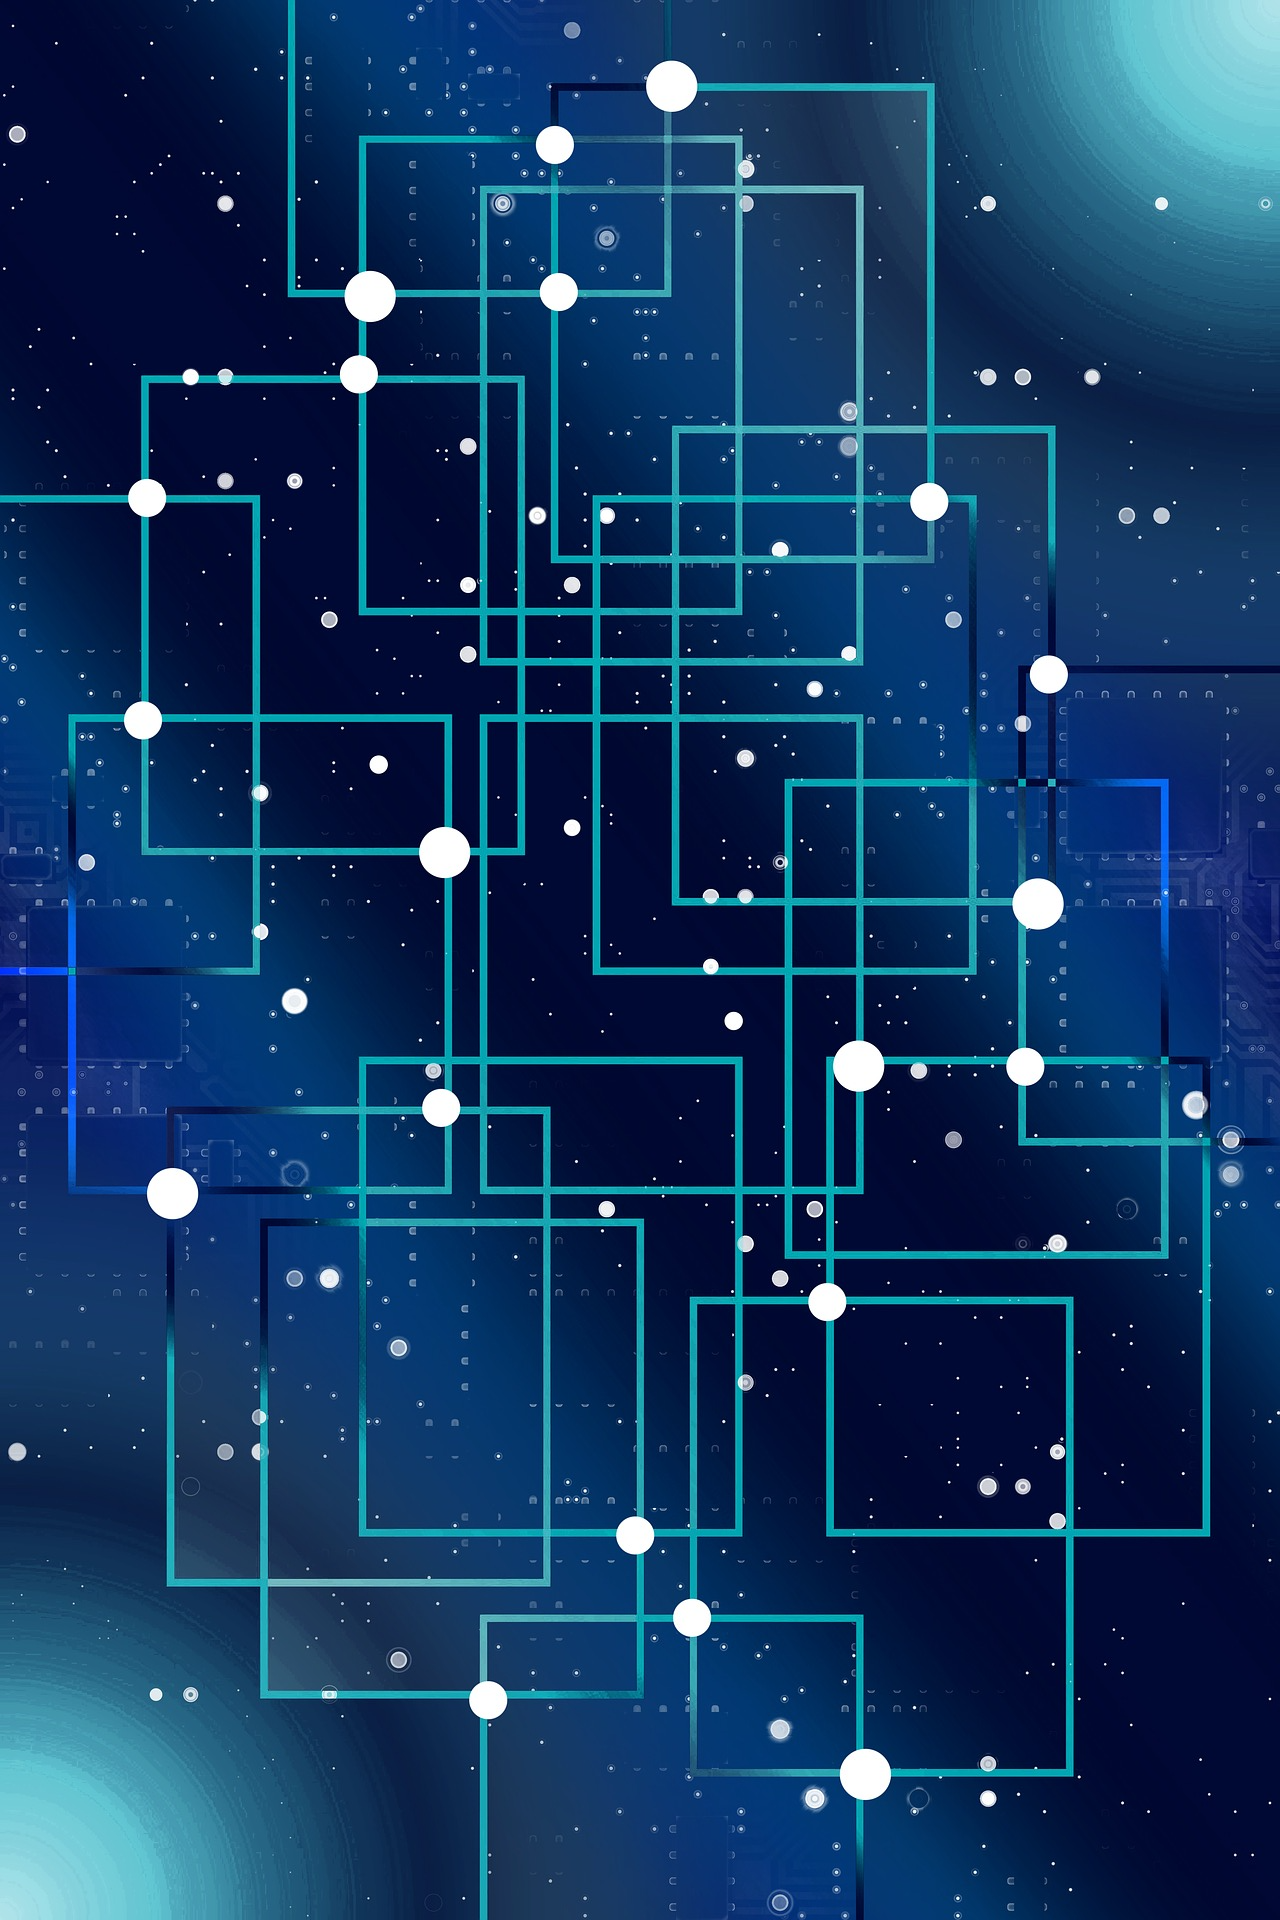
\includegraphics[width=\paperwidth]{background.png}};
\draw (current page.center) node [fill=blue!2!white,fill
opacity=0.9,text opacity=1,inner
sep=1cm]{\Huge\centering\bfseries\sffamily\parbox[c][][t]{\paperwidth}{\centering
    \TITLE \\[15pt] % Book title
    {\Large \SUBTITLE}\\[20pt] % Subtitle
    {\huge \AUTHOR \\ \Large \EMAIL} \\
    {\normalsize \TODAY} \\
    {\normalsize   \url{https://tinyurl.com/vonLaszewski-handbook} } \\
  }
}; % Author name
\end{tikzpicture}
\vfill
\endgroup

%----------------------------------------------------------------------------------------
%	COPYRIGHT PAGE
%----------------------------------------------------------------------------------------

\newpage
~\vfill
\thispagestyle{empty}

\noindent Copyright \copyright\ 2017\\
\AUTHOR \\

\noindent \EMAIL \\ % Copyright notice

% \noindent \textsc{Indiana University}\\ % Publisher

\noindent \url{https://github.com/cloudmesh/classes}\\

\noindent \url{https://tinyurl.com/vonLaszewski-handbook}\\


\begin{comment}
\noindent Licensed under the Creative Commons
Attribution-NonCommercial 3.0 Unported License (the ``License''). You
may not use this file except in compliance with the License. You may
obtain a copy of the License at
\url{http://creativecommons.org/licenses/by-nc/3.0}. Unless required
by applicable law or agreed to in writing, software distributed under
the License is distributed on an \textsc{``as is'' basis, without
  warranties or conditions of any kind}, either express or
implied. See the License for the specific language governing
permissions and limitations under the License.\\ % License information

\end{comment}

\noindent \textit{First printing by Gregor von Laszewski, October 2017} % Printing/edition date

%----------------------------------------------------------------------------------------
%	TABLE OF CONTENTS
%----------------------------------------------------------------------------------------

%\usechapterimagefalse % If you don't want to include a chapter image, use this to toggle images off - it can be enabled later with \usechapterimagetrue

\chapterimage{TOC.png} % Table of contents heading image

\pagestyle{empty} % No headers

\shorttableofcontents{Short Table Of Contents}{0}
\newpage
\tableofcontents % Print the table of contents itself

\cleardoublepage % Forces the first chapter to start on an odd page so it's on the right

\pagestyle{fancy} % Print headers again



